\documentclass[10pt,conference,compsocconf,letterpaper]{IEEEtran}
\usepackage{graphicx}

\begin{document}
\title{Federated Consistency in Geographically Distributed Systems}
\author{\IEEEauthorblockN{Benjamin Bengfort and Pete Keleher}
\IEEEauthorblockA{Department of Computer Science\\
University of Maryland, College Park, MD, USA\\
\{bengfort,keleher\}@cs.umd.edu}}


\date{September 1, 2016}

\IEEEtitleabstractindextext{%
\begin{abstract}
Consistency in a distributed storage system is usually thought of as one of a few discrete categories: eventual, causal, sequential, or linearizable and distributed systems are designed with homogenous replica types to fit one of those categories. In this paper we present Federated Consistency, a heterogenous system model that allows individual replica servers to select their own consistency level, specifying a quality of service at a particular location while still providing global guarantees. This model, applied to variable latency geographic systems that are partition prone allow for flexibility in consistency that can adapt in response to the local network environment.
\end{abstract}}

\maketitle

\IEEEdisplaynotcompsoctitleabstractindextext

\section{Introduction}

The rise of on-demand computing resources and the Cloud have made distributed systems the default approach to scaling applications for many users in a variety of geographic locations. In particular, data replication is used to increase availability, throughput, durability, and fault tolerance by ensuring that objects can be accessed on multiple servers as locally as possible. Although some coordination is necessary to ensure that replication happens correctly, many systems favor a relaxation in consistency in order to meet the performance requirements of modern, mobile applications. This is partially because the application layer can define its own mechanisms for handling differently consistent behavior, but it is primarily because such systems are implemented in data center contexts that enjoy stable, low latency connections which provide the opportunity for optimistic techniques via extremely low per-object inconsistency periods \cite{bailis_quantifying_2014,bermbach_metastorage:_2011}.

We might, therefore, generally categorize most modern distributed storage systems and NoSQL databases as not having strong consistency and using some consensus algorithm for control and synchronization when necessary. As a result consistency is usually described in a discrete, data-centric fashion: weak or strong; eventual, causal, or sequential and no longer described in client-centric terms \cite{bermbach_consistency_2013}. As replication becomes more prevalent, however, it is not enough to simply lay the burden of conflict at the feet of clients and there has been recent interest in instead redefining consistency along a spectrum whose dimensions are the strictness of ordering writes and the potential staleness of reads \cite{yu_design_2002,li_making_2012,afek_quasi-linearizability:_2010,al-ekram_multi-consistency_2010,krishnamurthy_adaptive_2002}.

By defining consistency in terms of ordering and staleness it is easy to see that the root cause of the tradeoff between performance and correctness is message latency, where a common case is when messages do not or cannot arrive due to node failure or network partitions. It has been noted that message latency is the key factor in determining ``how consistent'' a system is either due to staleness in eventually consistent systems \cite{bailis_probabilistically_2012} or by preventing progress in sequential consistency systems implemented with consensus \cite{howard_raft_2015}. The advent of distributed storage as a service has allowed systems to adapt consistency at runtime by taking advantage of a stable network environment \cite{chihoub_harmony:_2012,chihoub_consistency_2013,kraska_consistency_2009} and has shifted the focus away from replication in weakly-connected, dynamic, or mobile networks even though it is the environment that has the primary role in determining the behavior of replication and potential guarantees \cite{pitoura_data_1999,deno-toc}. We believe that local, user-oriented distributed systems should augment cloud services rather than be replaced by them; and in some cases, such as disaster recovery or search and rescue, may be the only available system.

In this paper we present a novel approach to flexible consistency via the federation of a heterogenous system of replica servers that implement a variety of consistency protocols in response to local policies and requirements. As a result, individual replicas in the system can respond and adapt to a changing network environment while providing as strong a local guarantee or minimum quality of service as required. The global state of a federated system is defined by the topology of replicas and their interactions, such that if a subset of nodes implement stronger consistency models, then the global probability of conflict is reduced and conversely if a subset of nodes implements weaker consistency then global throughput is increased. Indeed, we find that it is more often the tension between local vs global views of consistency that cause greatest concern in terms of application performance. Because each node can select and change local consistency policies, client applications local to the replica server have greater control of tuning consistency in response to mobile or dynamic network behavior, maximizing timeliness or correctness as needed.

We show that a federated consistency protocol finds a middle ground in the trade-off between performance and consistency, particularly between an eventually consistent system implemented via gossip-based anti-entropy \cite{kempe_gossip-based_2003} and a sequential consistency model implemented by the Raft consensus protocol \cite{ongaro_search_2014}. By exploring these two extremes in the consistency spectrum we show that the overall number of inconsistencies in the system is reduced from the homogenous eventual system and that the access latency is decreased from the homogenous sequential system. Moreover, because the global consistency of the system is topology-dependent, it can be said to have flexible or dynamic consistency. We have found that large systems with variable latency in different geographic regions can perform well by allowing most nodes to operate in an optimistic fashion, but maintain a strong central quorum to reduce the amount of global conflict.

The rest of the paper is organized as follows: we present a system model that is slightly different from the usual client-server system model and which has many more replica servers participating in a variety of locations. Because we take a client-centric approach we will describe a distributed file system, though our model can be easily generalized to other types of data systems. We will then present a consistency model to describe the impact of conflict, misordering, and staleness and use these metrics to next describe the federated consistency protocol. Finally we will present the performance of our system via experimental simulation and conclude with a discussion of how to adapt this model to include other consistency protocols like causal consistency.

\section{System Model}

In order to demonstrate the benefits of federation, we present a system model that shifts away from the traditional cloud-service oriented approach to distributed systems where clients connect to replica servers that may be geographically distributed but usually reside in data centers. We have found that this presentation usually involves many clients connecting to just a few replicas and we intend to discuss replication in medium to large systems with dozens or hundreds of replicas. Instead we present an approach where every client itself is a replica that accesses data locally, which it expects to be both as recent and as correct as possible. To that end we posit a file system as the natural use case of local, client-oriented systems, though we could easily generalize the model to any distributed storage system.

\subsection{Topology}

\begin{figure}[h]
    \centering
    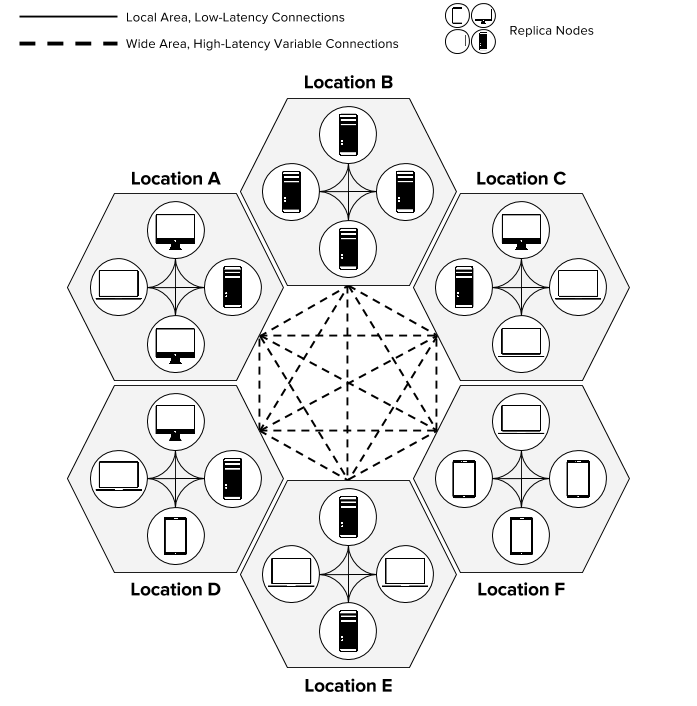
\includegraphics[width=0.5\textwidth]{figures/topology}
    \caption{A topology with many heterogenous replicas operating in a variable latency, partition and failure-prone environment.}
    \label{fig:topology}
\end{figure}

In order to investigate the effect of variable latency and the network environment on consistency, we have constructed a fully connected topology of replica nodes that are each assigned a geographic region as shown in Figure \ref{fig:topology}. Within each region, replica nodes enjoy stable, low-latency connections with their neighbors. However, across regions the latency is higher and the connections variable, meaning that out of order messages are more common across the wide area than in the local area.

In this type of topology there are two types of failure: node failure and network partitions. \textit{Node failure} occurs when a single node is shut off or stops responding to messages. \textit{Network partitions} occur when it is not possible for messages to be sent or received from a single geographic region. In both cases, two conditions must be dealt with by the replication protocol in order to satisfy correctness criteria: first the fact that accesses may continue at a partitioned node which are not being replicated by the system and second that the partitioned nodes are behind the global state and must be brought up to date.

\subsection{Logs and Accesses}

Because consistency is defined in terms of an ordering of operations that change the state of a replica, each node maintains a log of operations whose ordering and staleness can be reasoned upon. The question then becomes what those operations are in the context of a file system. A first attempt might be to map all reads and writes as individual operations that must be ordered, however that would be inefficient if the accesses are at the level of buffered system reads and writes. Instead, distributed systems usually aggregate individual accesses into \textit{Close-To-Open} (CTO) consistency where read and write accesses are ``whole file''. Furthermore, with respect to local accesses we must guarantee that a read returns the last write (given no remote updates, \textit{Read Your Writes Consistency}) and that writes are atomic with respect to each other (\textit{Monotonic Write Consistency}).

Each replica's log therefore is composed of a series of write accesses to multiple objects. Each object has a unique name that identifies it to the system and a monotonically increasing version number which can be implemented either as a vector clock \cite{parker_detection_1983} (or a simple Lamport scaler) in the case of a fixed topology or as a vector stamp \cite{almeida_version_2002} in the case of dynamic topologies. Therefore a write access encapsulate the following information: the name of the object being written to, the parent version of the object to which the write is being applied, the versions and object names of any other dependencies, the replica id where the write occurred, , and an array of blob ids that compose the file at the conclusion of the write.

A read access to a particular object simply looks up the latest local version of that object. Because dependency information can be embedded into a write, it is not necessary to include read accesses in the log. For example, in order to create a transaction that reads from objects $X$ and $Y$, performs a computation then updates objects $Y$ and then $Z$: the write to $Y$ would include as a dependency the earlier version of $Y$ and the read version of $X$ and the write to $Z$ would include the updated version of $Y$ and the read version of $X$. Other notions of dependencies include implicit session dependencies, e.g. all writes are dependent on any access that occur within a minimum time threshold of each other, or explicit dependencies that are added by the application.

Because our system model accounts for heterogenous devices and each write in the log is simply metadata about the version of a file we consider version replication as a separate issue from object or blob replication. Furthermore, system consistency depends only on the replication of version information since a version defines what is visible on each replica to be read (and writes follow an implicit read). While a version must become visible (replicated to) all devices in order for the system to be consistent, the blobs that make up data may not be stored on all devices with different storage resources. If a read access requires blobs that it doesn't have, it can simply request them from a local neighbor that does, or from the origin replica itself.

\section{Consistency Model}

\section{Federated Consistency}

\section{Simulation Results}

\section{Discussion}

\section{Related Work}

One of the earliest attempts to hybridize weak and strong consistency was a model for parallel programming on shared memory systems by Agrawal et al \cite{agrawal_mixed_1994}. This model allowed programmers to relax strong consistency in certain contexts with causal memory or pipelined random access in order to improve parallel performance of applications. Per-operation consistency was extended to distributed storage by the RedBlue consistency model of Li et al \cite{li_making_2012}. Here, replication operations are broken down into small, commutative suboperations that are classified as red (must be executed in the same order on all replicas) or blue (execution order can vary from site to site), so long as the dependencies of each suboperation are maintained. The consistency model is therefore global, specified by the red/blue ordering and can be adapted by redefining the ratio of red to blue operations, e.g. all blue operations is an eventually consistent system and all red is sequential.

The next level above per-operation consistency hybridization is called \textit{consistency rationing} wherein individual objects or groups of objects have different consistency levels applied to them to create a global quality of service guarantee. Kraska et al. \cite{kraska_consistency_2009} initially proposed consistency rationing be on a per-transaction basis by classifying objects in three tiers: eventual, adaptable, and linearizable. Objects in the first and last groups were automatically assigned transaction semantics that maintained that level of consistency; however objects assigned the adaptable categorization had their consistency policies switched at runtime based on a cost function that either minimized time or write costs depending on user preference. This allowed consistency in the adaptable tier to be flexible and responsive to usage.

Chihoub et al. extended the idea of consistency rationing and proposed limiting the number of stale reads or the automatic minimization of some consistency cost metric by using reporting and consistency levels already established in existing databases \cite{chihoub_harmony:_2012,chihoub_consistency_2013}. Here multiple consistency levels are being utilized, but only one consistency model is employed at any given time for all objects, relaxing or strengthening depending on observed costs. By utilizing all possible consistency semantics in the database, this model allows a greater spectrum of consistency guarantees that adapt at runtime.

Finally, Al-Ekram and Holt \cite{al-ekram_multi-consistency_2010} propose a middleware based scheme to allow multiple consistency models in a single distributed storage system. They identify a similar range of consistency models, but use a middleware layer to forward client requests to an available replica that maintains consistency at the lowest required criteria by the client. However, although their work can be extended to deploying several consistency models in one system, they still inspected homogenous consistency models being swapped out on demand as client requirements changed.

Continue with a discussion about conit, quasi-linearizability and continuous scale models.

\section{Conclusion}

\section*{Acknowledgments}

\bibliographystyle{plain}
\bibliography{references}


\end{document}
